\chapter{Calibration of the NOvA Test Beam Detector}\label{sec:TestBeamCalibration}

What to include from the technotes?

\section{The NOvA Test Beam Experiment}

Do I need to have this section? Maybe not...

\section{The NOvA Test Beam Detector}
Describe the test beam detector - copy from the technote

Describe the data and the selection - should this be a separate section?

\iffalse
\begin{figure}[hbtp]
\centering
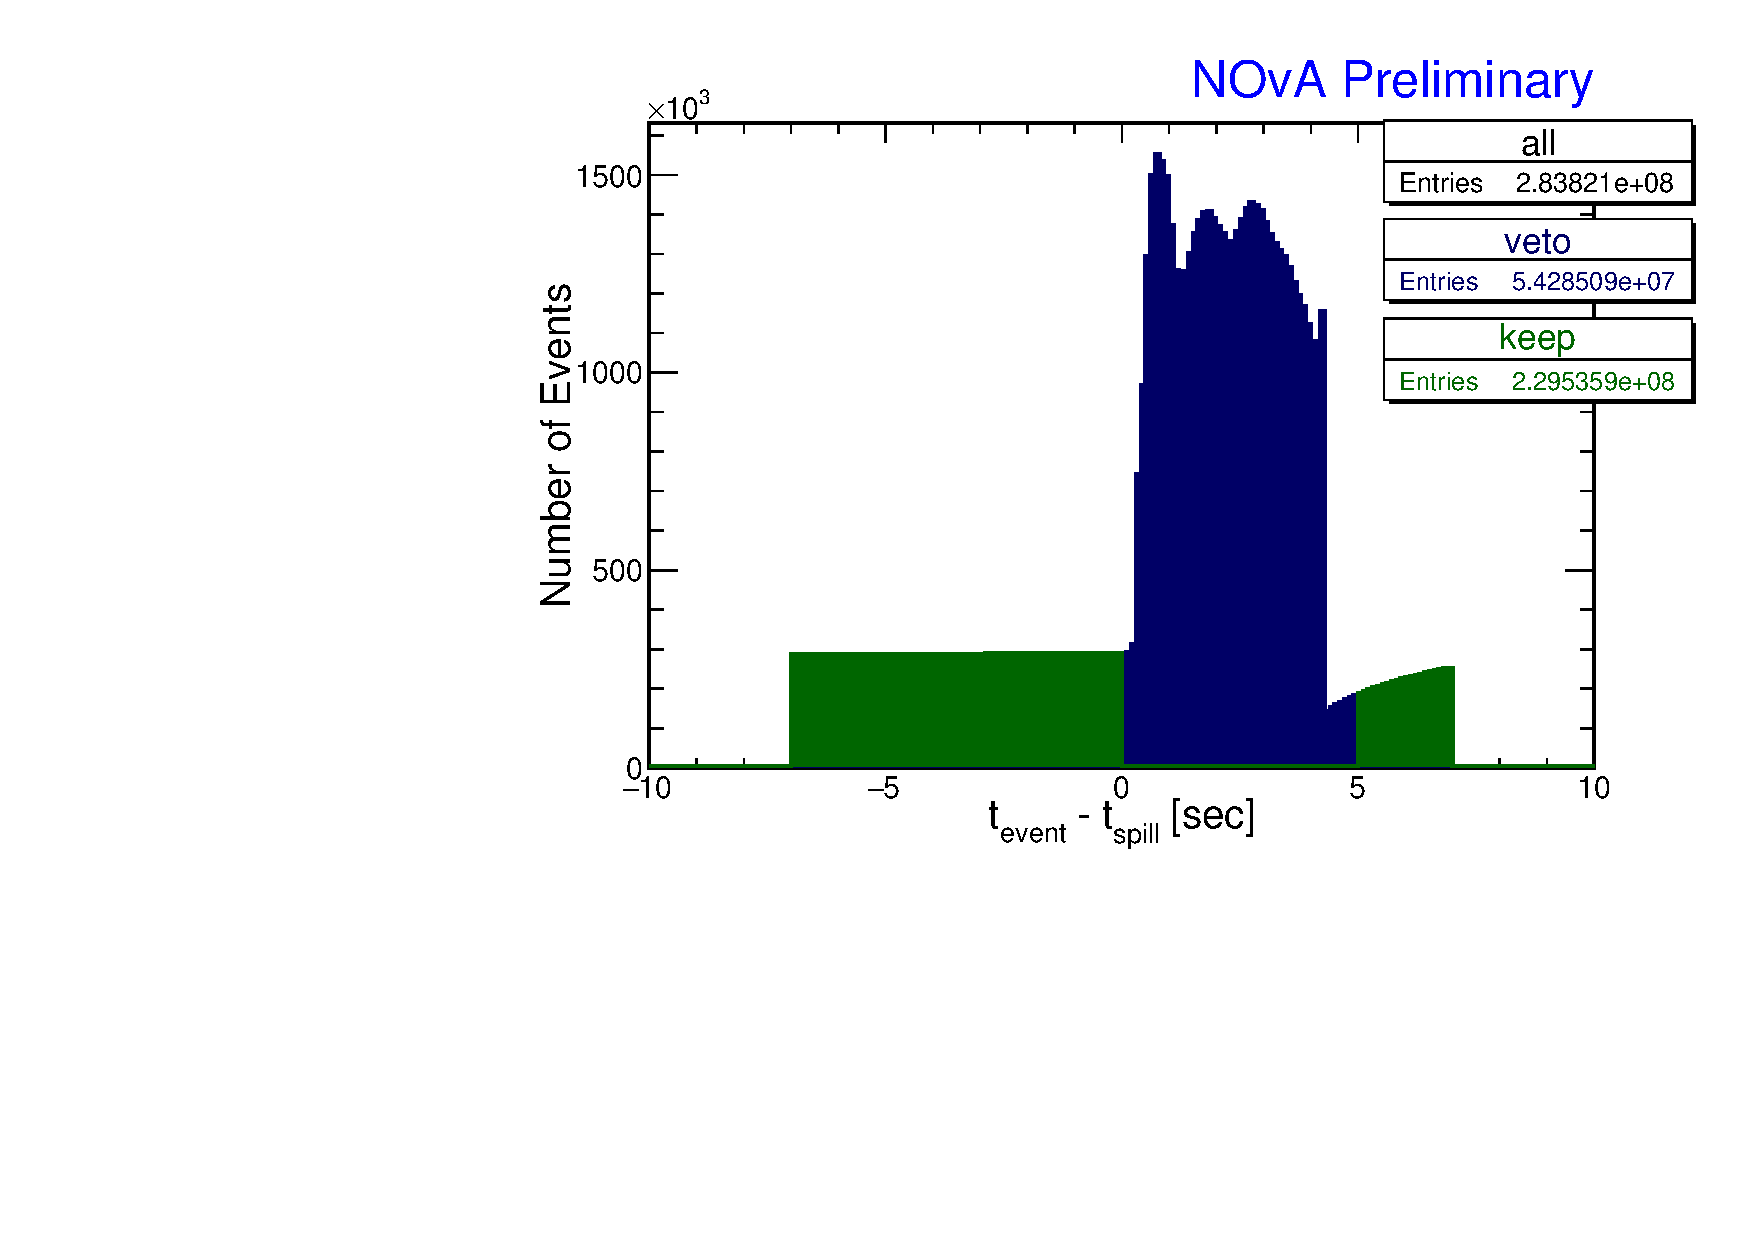
\includegraphics[width=\textwidth]{Plots/RemoveTBSpills.pdf}
\caption{Test Beam beam spill events removed from the calibration samples. Test Beam beam spill is 4.2 seconds long and we remove events (in blue) within a 5 seconds window from the start of the beam spill. The remaining events (green) should mostly consist of cosmic particles. This example and the numbers of entries are for the full period 4 Test Beam sample.}
\label{figRemoveBeamSpill}
\end{figure}
\fi

\section{Simulation of Cosmic Muons in the Test Beam Detector}
basically copy from the technote. Cite Teresa's thesis

\section{NOvA Test Beam Detector Calibration}
Basically copy from the technote.